\chapter{Reliability Analysis}
\chaptermark{Reliability}

The attempt to define the difference between \emph{reliability} and \emph{quality} will certainly fail, since given the intentional ambiguity in our definition of quality (Chapter~\ref{sec:introduction}).
For our purposes, however, this terminological matter will not bother us, since we will simply define reliability analysis to be the analysis of the \emph{time} to \emph{failure}.
We will also assume that ``time'' and ``failure'' are well defined and agreed upon.

We intuitively understand ``more reliable'' to mean ``lasts longer''. 
We should also consider, however, the case of a product that is designed to fail after some time, thus forcing the consumer to buy a new one. 
Some may say that a major hi-tech company named after a fruit employs this practice. 
Be it true or not, I hope we can agree that good knowledge of your product's life expectancy is a desirable. 

Reliability analysis involves the study of a probabilistic property of our product- its survival.
Any probabilistic model will require calibration to reality via data. 
This chapter thus introduces both the probability calculus typically used for reliability analysis, and some statistical considerations involved when fitting these models.
But before the fun begins, we need some definitions and terminology.



% survival function
% hazard rate
% estimating survival
% probability calculus
% accelerated life models



\section{Probabilistic Analysis}
% competing risk
% series model
% parallel/redundant model
% r out of n model
% standby model
% complex systems
% min-cut max-flow and inclusion-exclusion
% two-state vs. nultistate systems




\subsection{A Static View}

Let $\x_j \in \set{0,1}, j=1,\dots,p$ denote the state of the $j$'th component of a system, and $x=(x_1,\dots,x_p)$.

\begin{definition}[Structure Function]
The \emph{structure function}, $\struct=\struct(x):x \mapsto \set{0,1}$, is an indicator function of the state of the system.
\end{definition}

\begin{definition}[Series System]
A \emph{series system}, or \emph{serial system}, is one where all components need to function for the system to function: $$\struct(x)=\prod_{j=1}^{p}x_j.$$
\end{definition}
A reliability diagram of a series system is given in Figure~\ref{fig:series_system}.
\begin{figure}[ht]
\centering
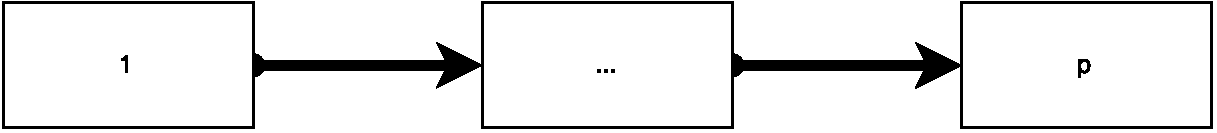
\includegraphics[width=0.5\linewidth]{art/series_system}
\caption{Series system.}
\label{fig:series_system}
\end{figure}


\begin{definition}[Parallel System]
A \emph{parallel system} is one where all components need to fail for the system to fail:
$$\struct(x)=1-\prod_{j=1}^{p} (1-x_j)= \coprod_{j=1}^p x_j.$$
\end{definition}
A reliability diagram of a parallel system is given in Figure~\ref{fig:parallel_system}.
\begin{figure}[ht]
\centering
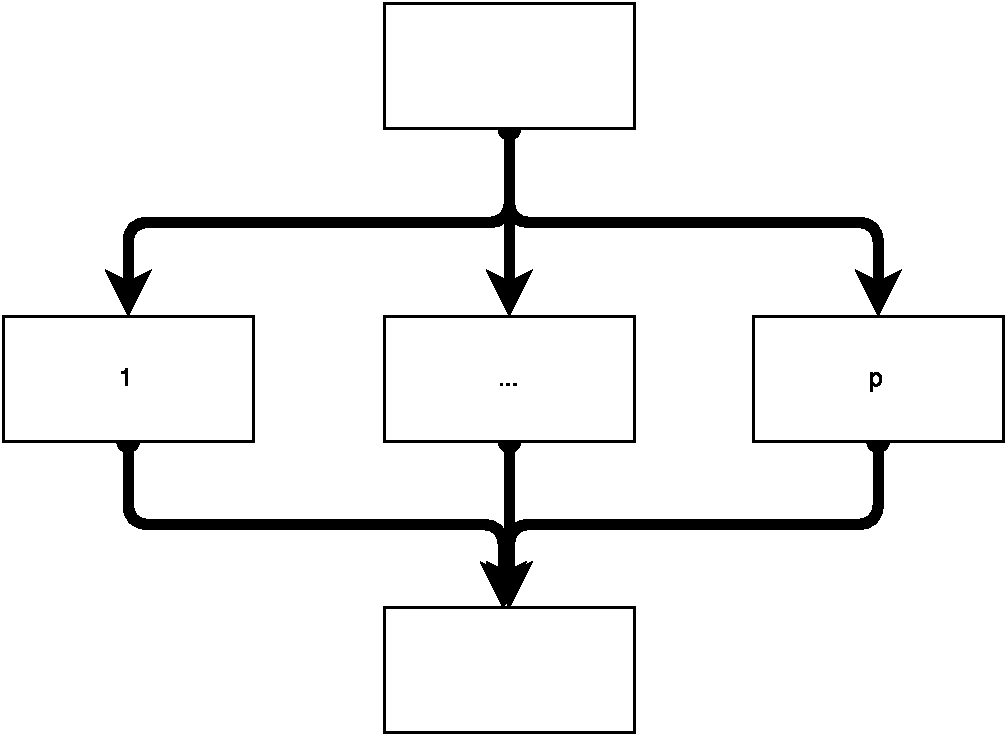
\includegraphics[width=0.5\linewidth]{art/parallel_system}
\caption{Parallel system.}
\label{fig:parallel_system}
\end{figure}


\begin{definition}[k-out-of-p System]
A \emph{k-out-of-p} system is one where at least $k+1$ components need to fail for the system to fail:
$$\struct(x)=\indicator{\sum_{j=1}^{p} x_j \geq k}.$$
\end{definition}
A reliability diagram of a k-our-of-p system is not provided, since it is not very friendly.




\begin{definition}[Monotone System]
A system is said to be \emph{monotone} if $\struct(x_1,\dots,\x_p)$ is non decreasing in all is components.
\end{definition}
The definition of monotonicity captures the idea that you cannot improve a system's state by breaking components.
This seems rather natural (I am still looking for a counter example).






\begin{definition}[Reliability]
We define the \emph{reliabity of component $j$} to be $$p_j:= P(\x_j=1),$$ 
and  the \emph{reliability of the system} 
$$ S_\struct:=P(\struct(x)=1).$$
\end{definition}


\begin{example}[Reliability of a series system]
For $\Phi(x)$ a series system, assuming independent components, we have
$$ S_\struct= \prod_{j=1}^{p} p_j.$$
\end{example}


\begin{example}[Reliability of a parallel system]
For $\Phi(x)$ a parallel system, assuming independent components, we have
$$ S_\struct= 1-\prod_{j=1}^{p} (1-p_j)= \coprod_{j=1}^p p_j. $$
\end{example}


\begin{example}[Reliability of a k-out-of-p system]
For $\Phi(x)$ a k-out-of-p system, assuming independent components with equal reliability ($p_i=p$), we have
$$ S_\struct= \sum_{i=k}^{p} \binom{n}{i} p^i (1-p)^{n-i} .$$
\end{example}


\begin{extra}[Reliability analysis of complex systems]
Except for simple systems, of the type we presented, the computation of the reliability of a complex system may be a formidable task. 
For complicated real-life systems, \emph{mix-cut--max-flow} algorithms, or \emph{inclusion-exclusion} type algorithms are emplyed. 
For more details, see \cite{aven_stochastic_1999}.
\end{extra}









\subsubsection{Reliability Importance Measures}
\begin{quotation}
The Strength Of The Chain Is In The Weakest Link.
\end{quotation}
This is obviously a profound observation in reliability analysis.
In order to identify the weakest link we require some measure of reliability importance.


\begin{definition}[Improvement potential]
The \emph{improvement potential} is defined as the change in a systems reliability, if we could force a component to function indefinitely.
Formally, we denote $\Phi^{(j)}$ to be a system where component $j$ cannot fail. 
We then define the improvement potential with respect to component $j$ to be 
\begin{align}
	I_j :=S_{\Phi^{(j)}}-S_{\Phi}.
\end{align}
\end{definition}



\begin{definition}[Birenbaum's measure]
\emph{Birenbaum's measure} is defined as the change in a systems reliability, if we infinitesimally improve the reliability of component $j$.
Formally 
\begin{align}
	I_j: =\frac{\partial}{\partial p_j} S_{\Phi}.
\end{align}
\end{definition}


Clearly any such importance measure, once computed, may serve to decide which component should be treated to improve reliability.







\subsection{A Time Dynamic View}
The reliability of each component ($p_j$), typically changes in time, and so does the reliability of the whole system.
In the following, $\T$ will typically stand for the time to malfunction. It is thus assumed to be \textbf{continuous} and \textbf{non-negative}.


\begin{definition}[CDF]
The cumulative distribution function (CDF) of a random variable $\T$ at a point $t$  is given by
\begin{align}
	\cdf{\T}{t}:= P(\T<t).
\end{align}
\end{definition}

\begin{definition}[PDF]
The probability density function (PDF) of a continuous random variable $\T$ at a point $t$ is given by 
\begin{align}
	\pdf{\T}{t}:= \frac{\partial}{\partial t}\cdf{\T}{t}.
\end{align}
\end{definition}


\begin{definition}[Survival Function]
The survival function of a random variable $\T$ at a point $t$ is given by 
\begin{align}
	\survive{\T}{t}:= P(\T>t)=1-\cdf{\T}{t}.
\end{align}
\end{definition}
By definition, it follows that if $\T_j$ is the time to failure of component $j$, then $p_j(t)=\survive{\T_j}{t}$.
Our notation bot $S_\struct$ also becomes clear, since it $\T_\struct$ is the time to failure of a structure $\Phi$, then we may write $S_\struct(t)=\survive{\T_\struct}{t}$.


\begin{example}[Survival of a series system]
For a series system $\struct$, the reliability of the system at time $t$ is given by $$\survive{\Phi}{t}=\prod_{j=1}^{p} p_j(t)$$.
\end{example}


\begin{example}[Survival of a parallel system]
For a series system $\struct$, the reliability of the system at time $t$ is given by $$\survive{\Phi}{t}=\prod_{j=1}^{p} p_j(t)$$.
\end{example}





Another way to present a distribution, no less informative than the previous ones, is by the \emph{hazard function}, which is the ``probability of surviving just another instant''.
\begin{definition}[Failure Rate]
The \emph{hazard function}, or \emph{failure rate}, of a random variable $\T$ at a point $t$ is given by \marginnote{Hazard Function}
\begin{align}
	\hazard{\T}{t} &:= \lim_{dt\to 0}\frac{P( \T \in [t,t+dt)|\T \geq t )}{dt} \label{eq:hazard}\\
	&= \frac{\pdf{\T}{t}}{\survive{\T}{t}} \\
	&= \frac{\partial}{\partial t}\log \survive{\T}{t}.
\end{align}
\end{definition}





\begin{definition}[Cumulative Risk]
The \emph{cumulative hazard}, \aka the \emph{cumulative risk}, of a random variable $\T$ at a point $t$ is given by \marginnote{Cumulative Hazrd}
\begin{align}
	\cuhazard{\T}{t} &:= \int_{0}^{t}\hazard{\T}{t} \\
	\Rightarrow \survive{\T}{t} &= \exp(-\cuhazard{\T}{t}). \label{eq:cumhazrd}
\end{align}
\end{definition}
Eq.(\ref{eq:cumhazrd}) readily shows that a distribution is well defined by its hazards.



\begin{theorem}[Failure rate of a series system]
The failure rate of a series system of independent components $\Phi$ is given by the sum of the failure rates of its components
\begin{align}
	\hazard{\Phi}{t}= \sum_{j=1}^{p} \hazard{\T_j}{t}
\end{align}
\end{theorem}
The proof is immediate using the cumulative risk.
The failure rate of a parallel system, does not admit such a nice closed form.




\begin{example}[Exponential Hazard]
The simplest distribution when discussing hazards is the exponential.
Recalling
\begin{align}
	\pdf{\T}{t}= \lambda \exp(-\lambda t) \indicator{t \geq 0} \\
	\cdf{\T}{t}= (1-\exp(-\lambda t)) 
\end{align}
so that 
\begin{align}
	\survive{\T}{t} &= \exp(-\lambda t), \\
	\hazard{\T}{t} &= \lambda.
\end{align}
\end{example}
The exponential is the only distribution with constant hazard which makes it very easy to analyze.
The constant hazard is due to the \emph{memoryless} property; think what the memoryless property implies on Eq.(\ref{eq:hazard}).



\begin{example}[Failure rate of a series of exponential components]
The failure rate of a series system $\Phi$, of $p$ independent components each with exponentially distributed failure times, is simply 
\begin{align}
	\hazard{\Phi}{t}= p \lambda, \forall t \geq 0
\end{align}
\end{example}
This is obviously the simplest system possible for reliability analysis, which stems from the fact that a minimum of exponentials is exponential with the sum of rates.



The following example, seemingly very simple, provides tremendous insight into the complexities of reliability analysis.
\begin{example}[Failure rate of a two exponential-component parallel-system]
\label{eg:failure_parallel}
Consider a system of two independent, parallel, exponential components, with failure times $\T_j\sim \exp(\lambda_j); j=1,2$.
The failure rate is given by
\begin{align}
	\hazard{\Phi}{t}=
	\frac
	{\exppdf{\lambda_1}{t} + \exppdf{\lambda_2}{t}  - \exppdf{(\lambda_1+ \lambda_2)}{t}}
	{\expcdf{\lambda_1}{t} + \expcdf{\lambda_2}{t} - \expcdf{(\lambda_1+ \lambda_2)}{t}}
\end{align}
\end{example}
Why is Example~\ref{eg:failure_parallel} so important?
Because it a very simple example in which the failure rate is no longer \textbf{non-monotone}, as depicted in Figure~\ref{fig:hazard_non_monotone}. 


\begin{figure}[ht]
\centering
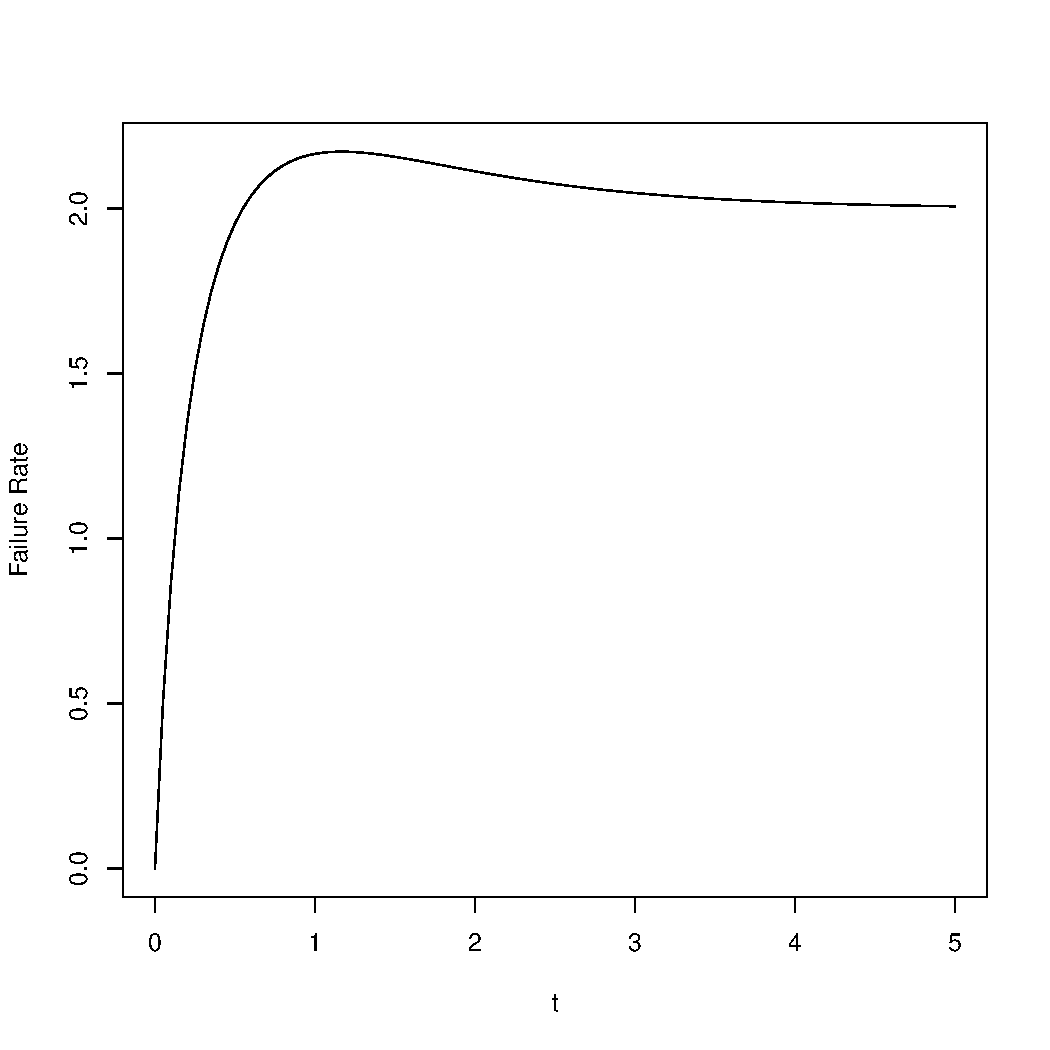
\includegraphics[width=0.5\linewidth]{art/hazard}
\caption{Failure rate of the parallel exponential component system.}
\label{fig:hazard_non_monotone}
\end{figure}





\begin{example}[Weibull Hazard]
The Weibull distribution is very common in reliability analysis, and can be constructed by 
$\T := \lambda \U^{1/k}$, where $\U \sim \exp(1)$. 
Recalling
\begin{align}
	\pdf{\T}{t} &= \frac{k}{\lambda}\left(\frac{\T}{\lambda} \right)^{k-1} \exp\left(-\frac{\T}{\lambda} \right)^k  \indicator{\T\geq 0} \\
	\cdf{\T}{t} &= 1 - \exp \left(-\frac{\T}{\lambda} \right)^k 
\end{align}
so that 
\begin{align}
	\survive{\T}{t} &= \exp \left(-\frac{\T}{\lambda} \right)^k \\
	\hazard{\T}{t} &= \frac{k}{\lambda} \left(\frac{\T}{\lambda} \right)^{k-1} .
\end{align}
\end{example}
Elementary analysis shows that the hazard function of the Weibull may be increasing or decreasing in time ($\T$), depending on $k$, but it is always monotone.




\begin{example}[Empirical risk rates]
When examining empirical risk rates of true devices, we almost always notice a \emph{bathtub} structure, such as in Figure~\ref{fig:bathtub}.
This shape captures the idea that products tend to fail more when they are brand new, or as they are very old, while their failure rates are fairly stable in the ``mid-life''.
In this text, we will not be providing a particular distribution which has this property. 
We refer the reader to \cite{nadarajah_bathtub-shaped_2008} for examples of distributions which have the bathtub property.
\end{example}


\begin{figure}[ht]
\centering
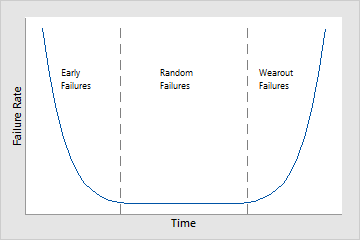
\includegraphics[width=0.5\linewidth]{art/bathtub_curve}
\caption{Bathtub curve of empirical failure rates. \newline
\url{http://support.minitab.com/en-us/minitab/17/topic-library/modeling-statistics/reliability/distributions-in-reliability-analysis/hazard-functions/}}
\label{fig:bathtub}
\end{figure}




\subsubsection{Aging}
The idea of \emph{aging} is an important one in reliability, as demonstrated by the empirical bathtub failure rate (Figure~\ref{fig:bathtub}).
Instead of checking if a particular distribution has some ageing property, we instead define classes of distributions with the desired notion of ageing.
Our goal will ultimately be to understand the reliability of a whole system, as a function of the reliability of its components.

\begin{definition}[IFR]
We call a failure time distribution to be in the \emph{increasing failure rate} (IFR) ageing class, if it has a non decreasing failure rate.
\end{definition}

Clearly IFR is not a strong enough notion of reliability, since we know from Example~\ref{eg:failure_parallel}, that two IFR components in parallel, are not an IFR system.


\begin{definition}[IFRA]
We call a failure time distribution to be in the \emph{increasing failure rate average} (IFRA) ageing class, if 
$\cuhazard{\T}{t}/t$ is non decreasing in $t$.
\end{definition}

\begin{definition}[NBU]
We call a failure time distribution to be in the \emph{new better then used} (NBU) ageing class, if 
$\survive{\T}{t_1+t_2} \leq \survive{\T}{t_2} \survive{\T}{t_1}$.
\end{definition}


\begin{definition}[NBUE]
Define the \emph{expected residual life}, $\mu(t)$, to be 
$$\mu(t):= \expect{\T-t|\T>t}.$$
\marginnote{Expected Residual Life}
We call a failure time distribution to be in the \emph{new better then used in expectation} (NBUE) ageing class, if 
$\mu(t) \leq \mu(0)$.
\end{definition}


\begin{theorem}
$IFR \Rightarrow IFRA \Rightarrow NBU \Rightarrow NBUE. $
\end{theorem}


The following theorem states a relation between the ageing properties of particular components, and that of the whole system. In particular it states that for the (very wide) class of monotone systems, then the IFRA property is conserved. 
This should be contrasted with the IFR property, which is not conserved, as demonstrated by Example~\ref{eg:failure_parallel}.
\begin{theorem}[IFRA closure theorem]
\label{thm:ifra_closure}
If the independent components of a monotone system are IFRA, then so is the whole system.
\end{theorem}



\begin{extra}[IFR and log-concave]
The IFR requirement, is essentially the same as log-concavity of the density function.
This immediately implies many properties of the class.
See \cite{bagnoli_log-concave_2005}.
\end{extra}



\begin{theorem}[Convolution of IFR]
For two independent random variables, $\x$ and $\y$, both in the IFR ageing class, then so is $\x+\y$.
\end{theorem}


\begin{example}[IFR of Gamma]
The Gamma (and thus the Erlang) distribution is in the IFR aging class, since it is the sum of exponentials, each in the IFR class.
\end{example}





\section{Statistical Analysis}
The probabilistic analysis of the previous section is great fun and all, but like any probabilistic problem, is has to be calibrated to real life. 
This is where data, and statistics come in.
Indeed, given any particular probabilistic model, we may write the likelihood problem, and call upon maximum likelihood principles.

The particular problems of failure data, we will have to work our way through are:
\begin{description}
\item [Identifiability] It is typically hard, if not impossible, to estimate the reliability of particular components, from the reliability of the whole system. 
\item [Censoring] a major concern with reliability data, is that in any finite length experiment, some events will just not have happened yet; their failure time will thus be censored. Ironically- the more reliable a component, the less data we will have to estimate its reliability. 
\item [Extrapolating from lab to life] Once estimated reliability in a lab, we would like to extrapolate findings into real-life operating conditions.
\item [Failure Distribution] like any statistical model, we will need to commit to some failure time sampling distribution.
\end{description}


\subsection{Identifiability}

\begin{example}[Likelihood estimation of a series system]
\label{eg:likelihood_of_failures}
Assume a series system $\Phi$ with $p$ independent, exponential components with rates $(\lambda_1,\dots,\lambda_p)$.
We have $n$ observations on the failure times of the system $t_1,\dots,t_n$.
How can we estimate the failure rates?
To use a likelihood approach, we need the data's sampling distribution.
Denoting the failure time of the $j$'th component of the $i$th device with $\T_{i,j}$, we have that $\T_{i,j}\sim \exp(\lambda_j)$ by assumption.
Since the system is serial, then $\T_i=\min_j(\T_{i,1},\dots,\T_{i,p})$.
By the properties of the exponential distribution $\T_i \sim \exp(\lambda)$, where $\lambda:=\sum_{j=1}^{p} \lambda_j$, as we have already seen with the failure rate. It follows that
$\pdf{\T_i}{t}=\lambda \exp(-\lambda t)$.
We may then write the likelihood function, maximize it with respect to $\lambda$ and discover, as we already know, that $$\hat{\lambda}=\frac{n}{\sum_{i=1}^{n} t_i}.$$
We are now left with the problem of recovering $(\lambda_1,\dots,\lambda_p)$ from $\lambda$. 
Can we do it? On the face of it- no. Which should not surprise us, since the mere knowledge of a device failure, is not very informative on the particular component that failed, which we would need to estimate $(\lambda_1,\dots,\lambda_p)$.
\end{example}

Example~\ref{eg:likelihood_of_failures} teaches us that unless further assumptions are introduced, the estimation of the component-wise failure rates requires information on the component-wise failure times. 





\subsection{Censor Events}
The problem of censoring, which in an extreme case may lead us to having no failure time data at all, will be approached in several ways. The first, will be an explicit modelling of censoring events.
The second, will be to introduce covariates, or factors in the DOE parlance, so that failure rates can be extrapolated from lab conditions, to operating conditions.


[TODO]





\subsection{Accelerated Life Models}
The \emph{accelerated life} model is very popular for very reliable components. This is because it may take forever to produce defect. We thus ``accelerate'' their life, by testing them under extreme conditions, and then scale back to the regular operating environment.

An accelerate life mode assumes that the effect of covariates are \textbf{multiplicative}. For this reason, a change in a covariate multiplies fail rates, as ``fast forwarding'' time would. 
Such models imply that 
\begin{align}
	\log \T = x'\beta + \varepsilon \Leftrightarrow \T = \exp(x'\beta) \times \T_0.
\end{align}
If $\T_1$ has $x_1'\beta=1$ , and $\T_2$ has $x_2'\beta=\gamma$, then 
\begin{align}
\survive{\T_2}{t}=\survive{\T_1}{t/\gamma},
\end{align}
which gives the model its name.

Popular accelerated time models include, that capture effects of temperature include the \emph{Arrhenius model}, and the \emph{Eyring model}.\marginnote{Arrhenius \\ Eyring}
For models for stress, voltage, humidity, and other life accelerating covariates, see \cite[Sec.8.1.5]{natrella_nist/sematech_2010}





\subsection{Proportional Hazard Models}
The \emph{proportional hazard}, or \emph{proportional risk} class of models, assumes that covariates multiply not survival times, but rather failure rates: 
\begin{align}
	\hazard{\T|x}{t}:=\hazard{\T|x_0}{t} \times \exp((x-x_0)'\beta) ,
\end{align}
where $x_0$ is some baseline condition with $\hazard{\T|x_0}{t}$ baseline hazard rate.
To fix idea, let $x \in \set{0,1}$ be a group indicator, in which case $\hazard{\T|x=1}{t} = \hazard{\T|x=0}{t} \exp(\beta)$, so that $\exp(\beta)$ can be interpreted as the \emph{relative risk}.\marginnote{Relative Risk}

The implied survival function satisfies $$ \survive{\T|x}{t}=\survive{\T|x_0}{t} \times \exp((x-x_0)'\beta).$$
In our two group example, a proportion hazard thus implies that group $x=1$ has $\exp(\beta)$ times more probability of surviving until time $t$ then group $x=0$. 


We may now ask ourselves, which of our favourite failure time distribution functions posses the accelerated life and the proportional hazard property. It turns out that the Weibull class is the only distribution with both properties.
We now explain for the particular instance of the exponential failure time distribution, which is part of the Weibull class.
\begin{example}[Accelerated life and proportional hazard in the exponential class]
Recall that the exponential distribution has a fixed failure rate (over time). 
If you change factors so that the \textbf{hazard doubles} (proportional hazard), it is still constant in time, thus exponentially distributed. 
If you accelerate life so that the \textbf{rate doubles} (accelerated life), it is still constant in time, thus exponentially distributed. 
\end{example}

%[HW: prove this for Weibull ]

\begin{extra}[General Hazard Rate Model]
The effects of covariates on the failure time distribution, may be modelled in many ways. 
The two models presented are probably the most popular, but may certainly be extended. 
For a more detailed discussion, see \cite{cox_analysis_1984}.
\end{extra}



\subsection{Choosing the Base Failure Rate}
Since the failure rate well defines the failure time distribution, and vise-versa, then choosing the base failure rate is the same as assuming the failure time distribution.
The three possible approaches include:
\begin{enumerate}
\item Assume a \textbf{parametric} model, such as exponential times, Weibull times, etc.
\item Assume a \textbf{semi-parametric} model, which can be simply seen as a flexible class of distributions, that has no particular parametric representation. In reliability analysis, the piece-wise constant hazard is a popular choice.
\item Do not assume anything on the distribution, known as a \textbf{non-parametric} proach. 
\end{enumerate}
If we assume a particular parametric model, then we may gather failure time data, write the likelihood function, and return failure rate estimates, and covariate effects.
We now focus on the more flexible framework of semi-parametric modelling.



\subsection{Piecewise Exponential Class}
Consider the proportional hazard model:
\begin{align}
	\hazard{\T|x}{t}:=\hazard{\T|x_0}{t} \times \exp((x-x_0)'\beta).
\end{align}
The model clearly requires some baseline failure rate $\hazard{0}{t}=\hazard{\T|x_0}{t}$.
A flexible, yet not too flexible assumptions, is that the failure rate is constant in some time intervals:
\begin{align}
	\hazard{0}{t}=h_j \quad \text{if} \quad t\in [\tau_{j-1},\tau_j)
\end{align}
This class of distributions clearly has $2J$ parameters: $(\tau_1,\dots,\tau_J,h_1,\dots,h_J)$.
We are free to choose $J$. Large $J$ are very flexible classes, but will require a lot of failure data to estimate.
Small $J$ are less flexible, but more easily estimable. At the limits, wen $J=1$, we are back to the exponential failure times. 

Since the failure rate is piece-wise constant, the distribution class is known as \emph{piece-wise exponential}.\marginnote{Piecewise Exponential}
It is a rather flexible class of distributions. Figure~\ref{fig:piecewise_exponential} depicts the approximation of the Weibull survival function, using a piece-wise constant hazard function, with $J=3$ and appropriate selected parameters.
\begin{figure}[ht]
\centering
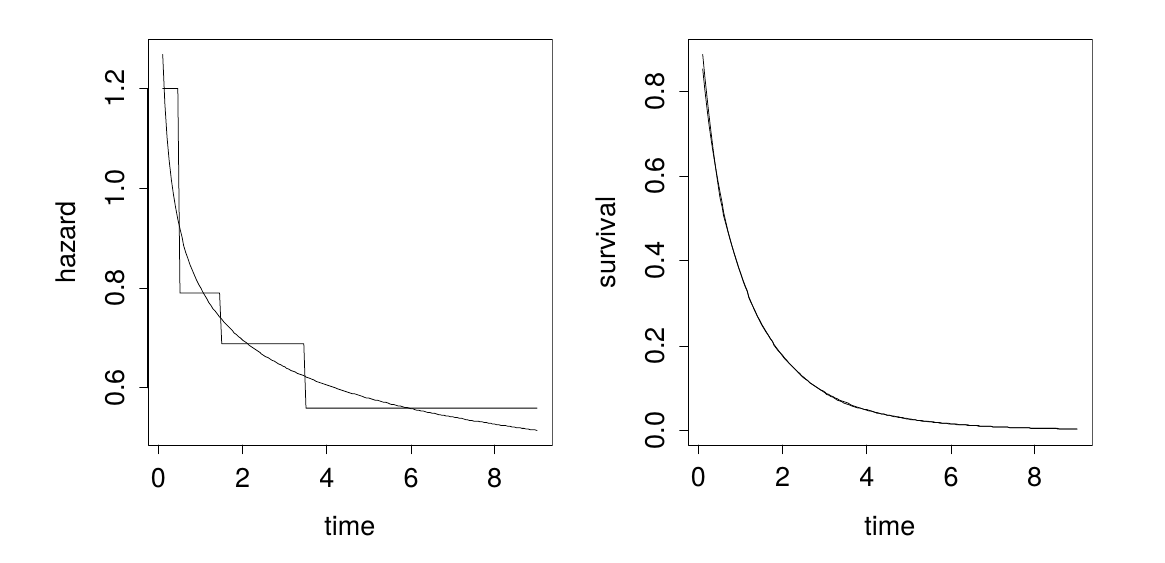
\includegraphics[height=0.2\textheight]{art/piecewise_exponential}
\caption{Piecewise Exponential aproximation of the Weibull distribution.}
\label{fig:piecewise_exponential}
\end{figure}





\section{Bibliographic Notes}
The probabilistic analysis is adapted from \cite{aven_stochastic_1999}.
The statistical analysis is adapted from German Rodriguez's Generalized-Linear-Models class notes\footnote{\url{http://data.princeton.edu/wws509/notes/c7.pdf}.} and \cite[Ch.8]{natrella_nist/sematech_2010}. 
An nice introductory discussion, may also be found in \cite{nahmias_production_2015}. 

